\section{Model}
\label{section:modele}

W sekcji tej znajdują się opisane modele, które zostały poddane eksperymentom numerycznym w projekcie. 
Opis modelu \texttt{STL} pokrywa się z tym, który został zamieszczony w dokumentacji wstępnej \cite{Dzienisz}, więc Czytelnik może pominąć sekcję \ref{subsection:stl}.
Jedyna różnica jaka między nim zachodzi polega na tym, że opis został rozszerzony o pseudokod algorytmów.

\subsection{Model lasu izolacyjnego}
\label{subsection:iforest}

Algorytm ten wybiera losową wartość podziału w przedziale między maksymalną a minimalną wartością cechy. w ten sposób dzielony jest cały zakres wartości cechy. W efekcie powstaje drzewo binarne w którym, ilość podziałów wymagana do wyizolowania próbki jest równa odległości od liścia do korzenia. Funkcją decyzyjną jest ta odległość, uśredniona względem drzew lasu. Jest ona miarą czy dana próbka jest anomalią czy nie.
  \[s(x, n) = 2^{\frac{-E(h(x)}{c(n)}}\]
  gdzie $E(h(x))$ jest uśrednioną względem wszystkich drzew długością ścieżki (ilością węzłów) prowadzącej od liścia do korzenia, $c(n)$ jest średnią długością ścieżki w drzewie, a $n$ jest ilością węzłów drzewa. \\
  Próbki będące anomaliami zwykle wymagają mniejszej ilości podziałów aby przejść z korzenia do liści. Gdy funkcja $s(x, n)$ osiąga wartości bliskie 1 to badany punkt z dużym prawdopodobieństwem jest anomalią, jeśli natomiast osiąga wartości bliskie 0.5 to punkt jest normalny.  \\
  
  Algorytm ten ma następujące parametry:
  \begin{itemize}
      \item rate Kontroluje on jaka część próbek średnio będzie uznawanych za anomalię. Przyjmuje wartości z zakresu $[0,1]$. Parametr ten zostanie dobrany eksperymentalnie. 
      \item ntrees - liczba wykorzystanych drzew 
      \item min-gain - minimalna zdobycz informacyjna konieczna żeby kontynuować podział
      \item prob-pick-avg-gain - prawdopodobieństwo podziału według atrybutu dającego największą średnia zdobycz informacyjną (wartość od 0 do 1)
      \item prob-pick-pooled-gain - prawdopodobieństwo podziału według atrybutu dającego największą łączną zdobycz informacyjną (wartość od 0 do 1) % nie wiem czy tak jest ok 
  \end{itemize}


\subsection{Model STL}
\label{subsection:stl}

Metoda STL (z ang. \emph{Seasonal-Trend decomposition using Loess})
opiera się na dekompozycji addytywnej szeregu czasowego na trzy składowe
w następującej formie

\begin{equation*}
x_{t} = \tau_{t} + s_{t} + r_{t},\; t = 1, \dots, N
\end{equation*}


gdzie \(x_{t}\) jest obserwowaną wartością szeregu czasowego,
\(\tau_{t}\) jest składową trendu, \(s_{t}\) składową sezonowości, a
\(r_{t}\) składową rezyduów. Dekompozycja taka jest dedykowana szeregom
czasowym z zauważalnymi wolnozmiennymi fluktuacjami sezonowości oraz
szybkozmienną składową trendu \cite{wen-gao}. Zakłada się
ponadto, że składowa rezyduów zawiera całą pozostałą informację o
szeregu czasowym -- m.in. szum. Można to sformalizować w następujący
sposób:

\begin{equation*}
  r_{t} = a_{t} + \epsilon_{t}
\end{equation*}


przy czym składowa \(\epsilon_{t}\) jest składową szumu, a \(a_{t}\)
modeluje poszukiwane anomalie w postaci nagłych przyrostów wartości
(t.zw. \emph{peak}'ów). Dekompozycja STL jest procedurą iteracyjną i
szczegółowo zostanie opisana w dokumentacji końcowej projektu. Na
potrzeby tego dokumentu należy zaznaczyć, że wynikiem dekompozycji jest
składowa \(a_{t}\), a składowa:

\begin{itemize}
\item
  szumu \(\epsilon_{t}\) jest usuwana wskutek operacji filtracji (ang.
  \emph{denoising}) przy pomocy średniej/mediany kroczącej lub
  probabilistycznemu wygładzaniu eksponencjalnego (PEWMA) \cite{PEWMA}
\item
  trendu \(\tau_{t}\) jest usuwana wskutek operacji detrendyzacji, która
  w najprostszym wariancie sprowadza się do zastosowania operatora
  różnicowego \begin{equation*} \nabla x_{t} = x_{t} - x_{t -1} \end{equation*}
    lub do filtrów kroczących
\item
  sezonowości \(s_{t}\), która jest usuwana w standardowej wersji
  metody STL przy pomocy LOESS (ang. \emph{locally estimated scatterplot
  smoothing}), tj. metody łączącej działanie średniej kroczącej z
  regresją wielomianową \cite{stl-origin}.
\end{itemize}

STL zawiera trzy parametry sterujące metodą:

\begin{enumerate}
\def\labelenumi{\arabic{enumi}.}
\item
  \(n_{p}\) liczbę obserwacji, która jest rozważana w każdym cyklu
  wyliczania składowej sezonowości
\item
  \(n_{i}\) liczbę iteracji wewnętrznej pętli algorytmu
\item
  \(n_{o}\) liczbę iteracji pętli zewnętrznej
\end{enumerate}

oraz trzy lub więcej parametrów sterujących detrendyzacją, usunięciem
szumu oraz ekstrakcją sezonowości.

Po otrzymaniu składowej \(a_{t}\) stosowany jest test (ang. Generalized Extreme Studentized Deviate test), który służy do wykrycia anomalii w badanym szeregu. Test ten stopniowo dostosowuje się do badanego szeregu przez wyrzucanie najbardziej odstających wartości i ponowne obliczanie wartości krytycznej. Przez odrzucenie kolejnych wartości zawyżających  ustala się wartość krytyczna. Test ten dostosowuje się przez parametr \[\alpha\] mówiący o szerokości wartości odstających do odrzucenia oraz przez procent anomalii spodziewanych w szeregu. Jest to metoda iteracyjna przez to jest bardziej czasochłonna niż np IQR jednak jest też bardziej odporna na wpływ wysokich anomalii.   


Dekompozycja szeregu czasowego przez algorytm STL znajduje się na
poniższym obrazku.

\begin{figure}[H]
\centering
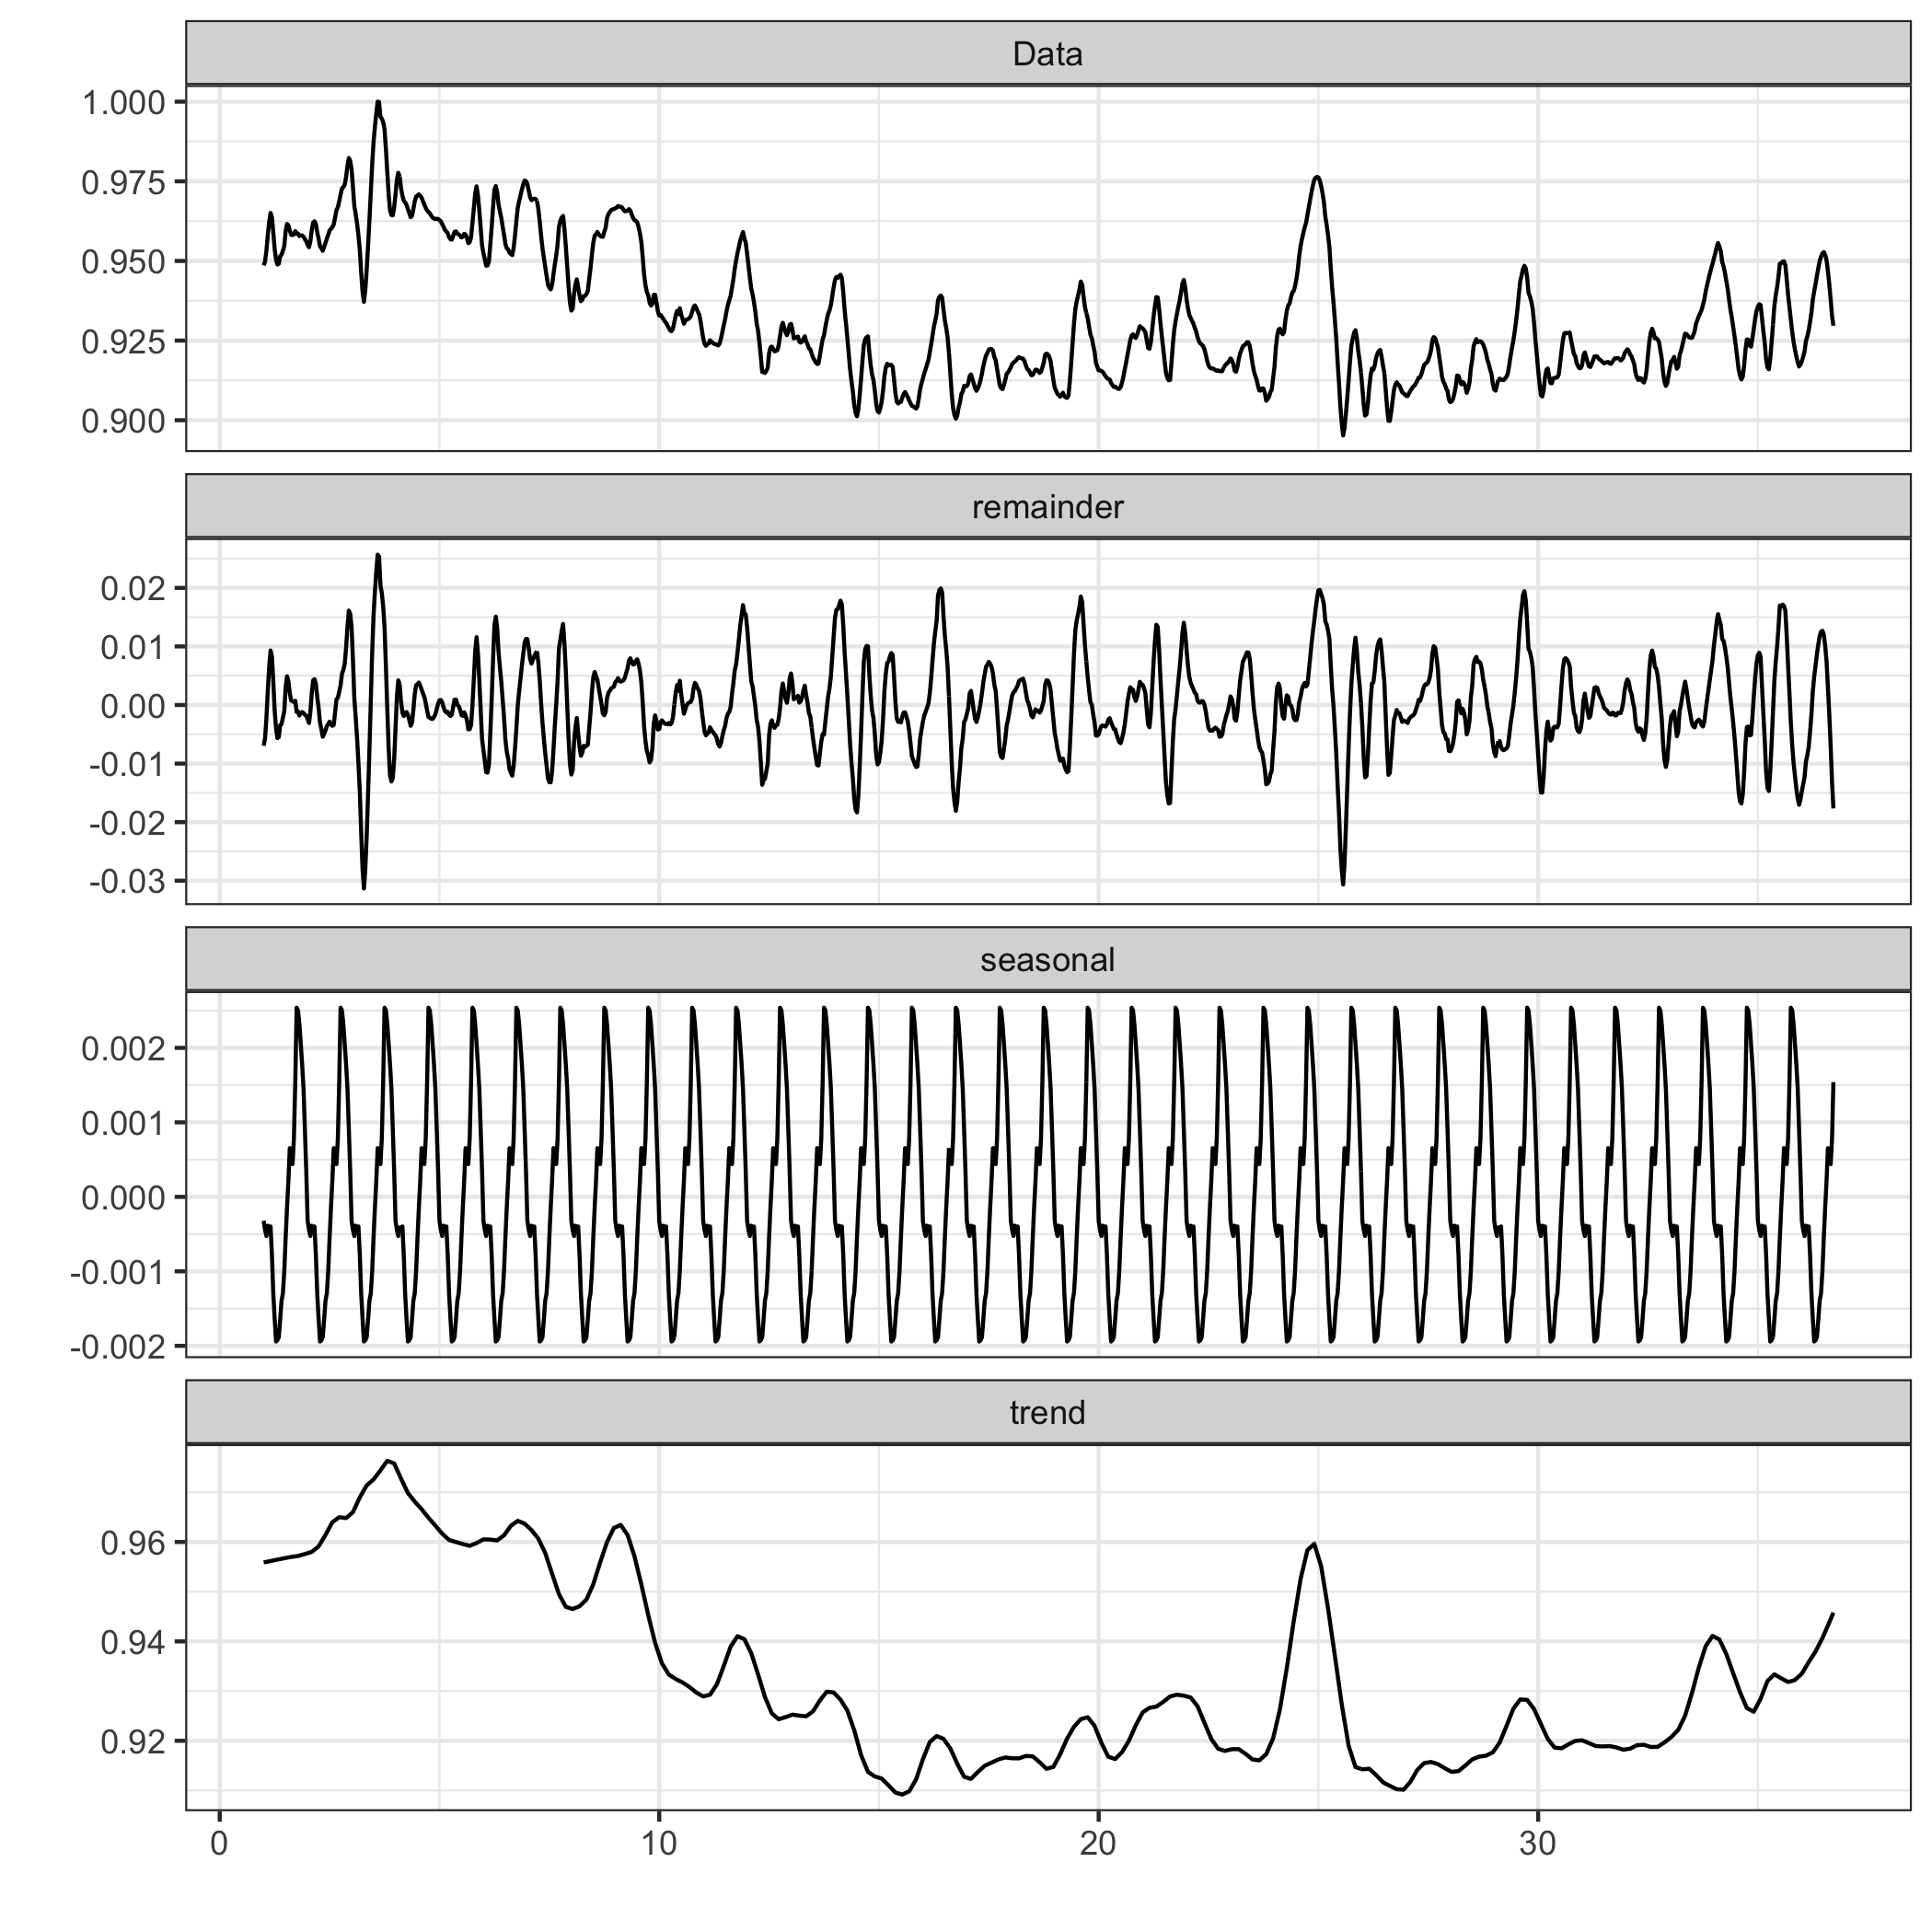
\includegraphics[width=\textwidth]{./images/stl-usage.png}
\caption{Dekompozycja szeregu czasowego metodą STL. Rysunek własny.}
\end{figure}

\subsection{Metody oparte na zanurzeniu szeregu czasowego w przestrzeni wielowymiarowej}

Algorytm bazuje na kroczącym oknie historii o długości $k$, które zanurza (ang. \emph{embed}) szereg czasowy w przestrzeni $k$-wymiarowej. Operacja taka umożliwia zastosowanie metod wielowymiarowych takich jak las izolacyjny, SVM lub LOF. Ważnym elementem występującym we wszystkich metodach tego typu jest dobór odpowiedniej wartości parametru $k$. Jeśli wartość $k$ będzie za mała algorytm będzie podatny na szum, natomiast jeśli $k$ będzie zbyt duże algorytm będzie niewrażliwy na lokalne anomalie. 


\subsection{Model OC-SVM}
\label{subsection:svm}

Jednoklasowy SVM (z ang. Support Vector Machine) jest nienadzorowaną metodą detekcji anomalii. 
\begin{equation}
    min_{w \in F, \bf{\xi} \in \mathbb{R}, \rho \in \mathbb{R}}\; x\ \frac{1}{2}||w||^{2} + \frac{1}{vl}\sum_{i} \xi_{i} - \rho 
    z ograniczeniami \text{subject to}\; (w\cdot\Psi(\textbf{x}_{i})) \geq \rho - \xi_{i}, \; \xi_{i} \leq 0
\end{equation}

Na podstawie tego równania wyznaczana jest funkcja $f$, która przyjmuje wartość 1 w niewielkim obszarze obejmującym znaczną część punktów (obszar gdzie punkty mają duże zagęszczenie) i wartość -1 w pozostałym obszarze. 
Dla nowych próbek wartość $f(x)$ wyznacza się poprzez decyzję, po której stronie hiperpłaszczyzny znajduje się ta próbka. 
Zbadane zostaną następujące parametry:
\begin{itemize}
    \item kernel - radialne jądro przekształcenia (parametr gamma)
    \item nu - jest skorelowany z górną granicą liczby źle klasyfikowanych przykładów i liczbą wektorów nośnych

\subsection{Model LOF}
\label{subsection:lof}

LOF (z ang. Local Outlier Factor) jest nienadzorowaną metodą detekcji anomalii. Dla każdego punktu wylicza ona lrd (z ang. local reachability density) w odniesianiu do punktów z jego sąsiedztwa.

\begin{equation}
    rld(p) = \frac{1}{\frac{\sum_{o \in N} reach-dist(p,o)}{|N(p)|}}
\end{equation}

gdzie $N$ jest sąsiedztwem punktu $p$. Zasięg punktu (z ang. reachability distance ) definiowany jest jako 
\begin{equation}
    reach-dist(p,o) = max(k-dist(o), d(p,o))
\end{equation}

gdzie $d(p, o)$ to odległość między punktami $p$ i $o$, a $k-dist$ jest to odległość między punktem $o$ a jego $k$-tym sąsiadem. Wartość ta mówi o tym jak daleko znajduje się punkt od kolejnego punktu w obszarze. Im mniejsza jest ta wartość tym większa odległość między punktami. 

Następnie na podstawie lrd danego punktu i wyników uzyskanych dla jego sąsiadów obliczany jest LOF 

\begin{equation}
    LOF(p) = \frac{\sum_{o \in N} \frac{lrd(o)}{lrd(p)}}{|N(p)|}
\end{equation}. 

Za anomalię uznawany jest punkt, którego zasięg jest znacznie mniejszy od zasięgów punktów sąsiedztwa. Ma to przełożenie na współczynnik LOF - dla punktów nieodstających uśrednione zasięgi dają wartości bliskie są 1 natomiast dla anomalii wartość ta jest znacznie większa od 1.  

Wybrany musi być próg \emph{tresh} od którego wartość zostanie uznana za anomalię oraz rozmiar okna \emph{k} w jakim anomalie będą badane.
